
%(BEGIN_QUESTION)
% Copyright 2007, Tony R. Kuphaldt, released under the Creative Commons Attribution License (v 1.0)
% This means you may do almost anything with this work of mine, so long as you give me proper credit

This illustration shows a diaphragm-operated pressure switch.  The ``impulse tube'' is the tube connecting process fluid pressure to the switch:

\vskip 50pt

$$\includegraphics[width=15.5cm]{i02968x01.eps}$$

Show how a voltage source and lamp would be connected to this switch to form a {\it high-pressure alarm}, turning the lamp on if the process pressure ever exceeds a certain set value.

\underbar{file i02968}
%(END_QUESTION)





%(BEGIN_ANSWER)

$$\includegraphics[width=15.5cm]{i02968x02.eps}$$

%(END_ANSWER)





%(BEGIN_NOTES)

%INDEX% Measurement, pressure: switch

%(END_NOTES)


